\pagestyle{plain} % No headers, just page numbers
% \pagenumbering{arabic} % Arabic numerals
% \setcounter{page}{1}


\chapter{\uppercase {Evaluation of the Deception Detection Capabilities of LLMs in Multimodal Settings}}

Deception detection, the ability to identify intentionally misleading intent, plays a critical role in safeguarding security, justice, and societal trust. Traditionally, its primary applications have been in criminalistics, particularly in interrogation and law enforcement settings such as suspect interrogations and security screenings. However, its relevance has expanded beyond these domains to border security~\cite{border}, healthcare~\cite{patient-doctor}, social media platforms~\cite{dd-social}, and consumer protection~\cite{opspam}. 

Despite its significance, deception detection remains inherently difficult, as human accuracy in detecting deception is only slightly above chance, $\sim54\%$~\cite{depaulo-54}. \textbf{Cognitive Load Theory}~\cite{vrij-clt} suggests that lying demands greater mental effort, which can lead to detectable inconsistencies, but deceivers often mitigate this by rehearsing or simplifying their fabrications~\cite{vrij2}. \textbf{Interpersonal Deception Theory}~\cite{buller-idt} highlights deception as an adaptive process, where deceivers adjust their behavior based on audience reactions, reducing the reliability of static detection methods. \cite{tdt} further explains humans’ bias toward assuming truthfulness, making them prone to overlooking deceptive cues. These challenges have driven the development of automated deception detection systems that systematically analyze linguistic, acoustic, and visual cues to improve reliability and scalability.

Researchers have increasingly explored automated approaches that combine advances in computer vision, natural language processing, and deep learning for deception detection. Early computational models in deception detection often relied on handcrafted features~\cite{Ekman2001, Zhang2020MultimodalDD, 8684170, Fan, Bai2019AutomaticLD}, drawing from facial micro-expressions, acoustic descriptors, and linguistic markers. With the emergence of deep learning, end-to-end architectures can directly learn deception-related patterns from raw multimodal data—text, audio, and video—leading to improved deception detection performance while reducing reliance on laborious feature engineering~\cite{dolos, SEPSIS, guo2024}. Despite these advances, existing deception detection systems still face challenges related to generalization, as deception cues vary across individuals, cultures, and contexts. Additionally, many deep learning models operate as black-box systems, making it unclear whether they genuinely capture deception-related patterns or rely on statistical shortcuts.

Recently, \textbf{Large Language Models (LLMs)} have demonstrated strong cognitive reasoning capabilities, excelling in tasks, such as emotion recognition~\cite{NEURIPS2024_c7f43ada, INSTERC, zhang-etal-2024-visual}, sentiment analysis~\cite{zhang-etal-2024-sentiment}, and fact verification~\cite{zhang-gao-2023-towards}. These models leverage large-scale pretraining and in-context learning to adapt to new tasks with minimal labeled data. LLMs’ ability to identify subtle linguistic cues, integrate multimodal inputs ~\cite{Chu2023QwenAudioAU, liu2023llava, zhang-etal-2023-video}, and and generate step-by-step reasoning behind the judgment through chain-of-thought prompting~\cite{cot} makes them promising candidates for automated deception detection. However, empirical evidence on LLM-driven deception detection, particularly in real-world multimodal settings, remains limited.

In this work, we take a comprehensive step toward filling this gap by challenging state-of-the-art LLMs with multiple deception detection tasks spanning three well-established datasets- \textbf{Real-life Trial Dataset, RLTD}~\cite{rltd}, \textbf{Miami University Deception Detection Database, MU3D}~\cite{mu3d}, and \textbf{Opinion Spam Dataset, OpSpam}~\cite{opspam}. These datasets cover deception across online, controlled, and real-world legal settings, collectively capturing diverse deception strategies and manifestations.

\section{Background}

\subsection{Problem Definition}

Deception detection is the task of identifying whether a statement or behavior is deliberately misleading. We define this task as a binary classification problem, where the goal is to predict \( y \in \{\texttt{Truthful}, \texttt{Deceptive}\} \) given an input processed by a large language model. Formally, let \( p \) denote a task-specific prompt that instructs the model to process the input content and generate the classification label as either truthful or deceptive, and let \( t \) represent the textual content under analysis (for instance, a speech transcript or an online review). In the simplest setting, the input is
\(
x = p \,\odot\, t,
\)
where \(\odot\) denotes concatenation, and the model generates the prediction via
\(
y = f_\theta(x),
\)
where $f_\theta$ represents the LLM parameterized by $\theta$. 

Although textual cues can be highly informative for deception detection, additional cues may arise from non-verbal or multimodal sources. To account for such signals, we allow the input to be augmented by auxiliary features \( u \), which could include descriptive text of facial expressions and body movements, or a textual summary of the observed video content or speech characteristics. In that case, the model processes
\(
x = p \,\odot\, t \,\odot\, u.
\)
Furthermore, when employing large multimodal models (LMMs) with the capacity of handling audio or video, the input can incorporate raw audio or video directly, denoted by \( a \) and \( v \) respectively, such that
\(
x = p \,\odot\, t \,\odot\, [a, v]
\)

\subsection{Datasets}

\textbf{Real-life Trial Dataset (RLTD)}: ~\cite{rltd} is constructed from publicly available courtroom trial recordings. Labels are assigned based on trial outcomes, with guilty verdicts indicating deception and non-guilty verdicts or exoneration indicating truthfulness. In some cases, the same individual contributes both deceptive and truthful statements, capturing within-subject deception variations. The dataset includes 121 video clips (60 truthful and 61 deceptive) with transcripts. The videos are also annotated for non-verbal features using the MUMIN multimodal coding scheme~\cite{mumin}, focusing on facial expressions, gaze, head, and hand movements.

\textbf{Miami University Deception Detection Database (MU3D)}: ~\cite{mu3d} is a controlled deception dataset capturing instructed deception in interpersonal scenarios. Participants were asked to describe individuals they liked or disliked while alternating between truthfulness and deception. The dataset comprises 320 (160 truthful and 160 deceptive) videos with metadata, including trustworthiness ratings, anxiety ratings, demographic details, and full speech transcriptions.

\textbf{Opinion Spam Dataset (OpSpam)}: ~\cite{opspam} focuses on deception in online reviews and consists of 1600 reviews evenly split between truthful and deceptive opinions about hotels. Deceptive reviews were artificially generated by paid participants instructed to write persuasive but fabricated reviews, while truthful reviews were collected from genuine user feedback on platforms like TripAdvisor and Yelp. The dataset presents a linguistic deception challenge where fabricated narratives must be distinguished from authentic experiences.

Together, these datasets provide a rigorous benchmark for evaluating LLMs and LMMs in deception detection across legal, interpersonal, and online domains, ensuring a comprehensive assessment of their effectiveness.

\subsection{Baselines}
We evaluate the LLM based approaches against several deep-learning and transformer based baselines for text-only and multimodal deception detection. For the baselines, we extract modality-specific features using state-of-the-art pre-trained encoders. We obtain textual features from the final hidden states of the RoBERTa-base~\cite{roberta} model. For acoustic features, we use the final encoder hidden states of the Whisper-base~\cite{whisper} model, which has demonstrated robust performance in various audio tasks~\cite{miah, whisper2}. For visual features, we sample the input video at 30 fps and encode each frame using CLIP~\cite{CLIP}. 

We consider four baselines to compare against LLM-based approaches. First, we implement a text-only baseline by fine-tuning RoBERTa with a two-layer MLP classification head. Second, we follow ~\cite{bilstm} to employ a Bi-LSTM with attention network on the multimodal features described previously. We concatenate the resulting representations from each modality and use linear layers for multimodal classification. In unimodal scenarios, we simply predict the label from unimodal representations. Third, we follow  ~\cite{cnn1, DL4} to use CNN with global average pooling for feature encoding. Again, we concatenate the features across all modalities for multimodal deception detection. Finally, we replicate the Parameter-Efficient Crossmodal Learning (PECL) model proposed in  ~\cite{dolos}, which uses a 1D-convolution-based temporal adapter to learn modality-specific temporal attention alongside pre-trained Wav2Vec2 and ViT backbone models, supplemented by a Plug-in Audio-Visual Fusion (PAVF) module for crossmodal attention. This design enables PECL to achieve strong performance in the audio-visual setting. We conduct all experiments using stratified \textbf{4-fold cross-validation} across all three datasets.



\section{Experimentatal Configurations}

We evaluate three Large Language Models (LLMs) for their deception detection capabilities: LLaMA3.1-8B~\cite{llama3.1}, Gemma2-9B~\cite{gemma2}, and GPT-4o~\cite{gpt4o}. Additionally, we assess the performance of various Large Multimodal Models (LMMs), categorized based on their modality specialization. For video-language models, we consider LLaVA-NEXT-Video~\cite{llavanextvideo} and Qwen2VL~\cite{qwen2vl}, while MERaLiON-AudioLLM~\cite{meralion} and Qwen2-Audio~\cite{qwen2audio} serve as the audio-language models. These models represent state-of-the-art architectures in language and multimodal understanding, offering a diverse perspective on deception detection across textual, audio, and visual modalities.

We evaluate both zero-shot and few-shot inference setups. In zero-shot evaluation, the model receives only a task description prompt and input data without labeled examples. In few-shot evaluation, the model is provided with a set of labeled examples for in-context learning. Specifically we have experimented with \( n = \{2, 4, 6, 8, 10\} \), as number of in-context examples. Under the zero-shot and few-shot setups, we experiment with various strategies and configurations, outlined below.

\subsection{Response Generation Strategies}
To systematically assess deception detection performance, We investigate two different response generation strategies: \textbf{direct label prediction}, where the model directly generates the label for the input as either \texttt{Truthful} or \texttt{Deceptive} without additional reasoning, and \textbf{post-hoc reasoning generation}, where the model is prompted to first generate the classification label \( y \) and then provide a justification \( r \), such that: \(
(y, r) = f_{\theta}(x) \),  where \( x \) is the input and \( f_{\theta} \) represents the model parameterized by \( \theta \). The generated reasoning \( r \) serves as a justification for the classification decision, allowing for better interpretability of deception detection outcomes. We also evaluate the chain-of-thought prompting for reasoning generation. However, post-hoc reasoning generation is eventually adapted for better performance and interpretability, with further analysis provided in Appendix~\ref{cot}.

\subsection{In-Context Example Selection Strategies}
For the few-shot prompting setup, we explore different strategies for selecting in-context examples. Similar to the baselines, we employ a 4-fold split for in-context example selection. The random selection approach involves choosing an equal number of truthful and deceptive examples randomly from the other 3 splits. In contrast, the similarity-based selection methods employ sentence-transformers to encode the target input and dataset samples, allowing for similarity-based retrieval. Within this method, we examine two variants: \textbf{sim-top}, which selects the most similar examples irrespective of their label, and \textbf{sim-pair}, which ensures a balanced selection of truthful and deceptive examples based on similarity ranking.

\subsection{Auxiliary Features}
We incorporate additional auxiliary features on top of the textual contents in the multimodal datasets, that provide valuable non-verbal and contextual information. As a first set of features for the RLTD dataset, we include a curated selection of 16 non-verbal features, capturing facial expressions and body movements indicative of deceptive behavior. The features names are listed in Appendix \ref{non-verbal}.  These features allow the model to leverage fine-grained behavioral cues that are often imperceptible in textual analysis alone. In addition to non-verbal gestures, we experiment with video and audio summaries as auxiliary inputs. A video-language model, LLaVA-NeXT-Video is employed to generate summaries of the visual content, extracting key information regarding speaker posture, facial expressions, and body movements indicative of stress or deception. Similarly, an audio-language model, Qwen2-Audio is used to summarize the tonal and acoustic features of the speech, identifying variations in pitch, intonation, and vocal stress patterns. These summaries provide a higher-level contextual representation of the non-verbal elements within the dataset, aiding in deception detection by supplying a multimodal understanding of deceptive cues for the RLTD and MU3D datasets.

\subsection{Fine-Tuning}
To further enhance model performance, we fine-tune open-source LLMs using the LLaMA-Factory~\cite{llamafactory} framework. We specifically fine-tune LLaMA3.1-8B, Gemma2-9B, and Qwen2-VL-7B. This fine-tuning process allows the models to better adapt to the nuances of deception detection by learning from domain-specific patterns and optimizing their ability to process multimodal cues effectively. 



\begin{table}[h!]
\centering
\footnotesize
\begin{tabular}{l c c cc cc cc}  % <-- Added an extra 'c' for the new 'Config' column
\toprule
\multirow{2}{*}{\textbf{Model}} 
  & \multirow{2}{*}{\textbf{Config}} 
  & \multirow{2}{*}{\textbf{Modality}} 
  & \multicolumn{2}{c}{\textbf{RLTD}} 
  & \multicolumn{2}{c}{\textbf{MU3D}} 
  & \multicolumn{2}{c}{\textbf{OpSpam}} \\
  \cmidrule(lr){4-5}\cmidrule(lr){6-7}\cmidrule(lr){8-9}
& & & \textbf{Acc} & \textbf{F1} & \textbf{Acc} & \textbf{F1} & \textbf{Acc} & \textbf{F1} \\
\midrule
\multicolumn{9}{c}{\textbf{Baselines}} \\  % <-- New row with "Baselines" centered
\midrule
RoBERTa-ft 
  & - & t        & 76.31 & 76.22 & \textbf{67.92} & \textbf{67.81} & 88.10 & 88.09 \\
\midrule
\multirow{4}{*}{BiLSTM+Attention}
  & \multirow{4}{*}{-} & t        & 69.42 & 69.37 & 65.94 & 65.76 & \underline{90.45} & \underline{90.45} \\
  &                    & a        & 68.04 & 68.02 & 62.19 & 61.82 & -     & -     \\
  &                    & v        & 75.48 & 75.38 & 55.21 & 55.11 & -     & -     \\
  &                    & t, a, v  & 77.14 & 77.04 & 62.29 & 62.19 & -     & -     \\
\midrule
\multirow{4}{*}{CNN}
  & \multirow{4}{*}{-} & t        & 64.46 & 64.39 & 64.06 & 63.91 & 86.37 & 86.36 \\
  &                    & a        & 60.88 & 60.13 & 60.42 & 60.26 & -     & -     \\
  &                    & v        & \underline{82.09} & \underline{82.09} & 54.06 & 53.95 & -     & -     \\
  &                    & t, a, v  & \textbf{83.47} & \textbf{83.44} & 60.41 & 60.38 & -     & -     \\
\midrule
PECL 
  & - & a, v      & 80.17 & 80.13 & 56.56 & 56.56 & -     & -     \\
\midrule
\multicolumn{9}{c}{\textbf{LLM Inference}} \\
\midrule
%--- Single-row LLMs (Few shot, t) ---
LLaMA 3.1 & Few shot & t & 71.69 & 77.11 & 57.03 & 56.84 & 62.93 & 62.47 \\
\midrule
Gemma 2   & Few shot & t & 71.69 & 71.38 & 55.08 & 53.75 & 64.81 & 64.51 \\
\midrule
GPT-4o    & Few shot & t & 79.55 & 79.49 & 55.70 & 53.87 & 74.50 & 74.00 \\
\midrule
%--- Multi-row LLMs (Zero shot) ---
\multirow{2}{*}{LLaVA-NEXT-Video} & \multirow{2}{*}{Zero shot} & v     & 52.06 & 43.55 & 50.00 & 33.33 & - & - \\
&  & t, v  & 64.46 & 61.79 & 50.31 & 50.31 & - & - \\
\midrule
\multirow{2}{*}{Qwen2VL}          & \multirow{2}{*}{Zero shot} & v & 51.24 & 37.95 & 50.31 & 39.94 & - & - \\
&  & t, v  & 63.64 & 60.32 & 52.50 & 52.35 & - & - \\
\midrule
\multirow{2}{*}{MERaLiON-AudioLLM}& \multirow{2}{*}{Zero shot} & a     & 66.94 & 66.11 & 49.06 & 33.97 & - & - \\
&  & t, a  & 66.12 & 63.57 & 49.38 & 34.12 & - & - \\
\midrule
\multicolumn{9}{c}{\textbf{LLM Finetuning}} \\
\midrule
\multirow{2}{*}{LLaMA 3.1} & \multirow{2}{*}{-} & t & 69.63 & 69.62 & 57.74 & 57.58 & \textbf{92.25} & \textbf{92.24} \\
&                          & t, u   & 72.72 & 72.46 & - & - & - & - \\
\midrule
\multirow{2}{*}{Gemma 2}   & \multirow{2}{*}{-} & t     & 75.21 & 75.19 & \underline{66.56} & \underline{66.55} & 90.25 & 90.18 \\
&                          & t, u   & 75.21 & 75.17 & - & - & - & - \\
\midrule
\multirow{2}{*}{Qwen2VL}   & \multirow{2}{*}{-} & v     & 57.85 & 57.10 & 52.20 & 51.43 & - & - \\
&                          & t, v   & 71.90 & 71.90 & 56.25 & 53.51 & - & - \\
\bottomrule
\end{tabular}
%\captionsetup{font=scriptsize}
% \captionsetup{font=footnotesize}

%\caption{Comparison of Baselines and LLM-Based Evaluations Across Modalities (t: text, a: audio, v: video, u: non-verbal features)}
\caption{Comparison of Baselines and LLM Results Across Modalities (t: text, a: audio, v: video, u: non-verbal features)}

\label{tab:myresults}
\end{table}



\section{Results \& Analysis}


In Table~\ref{tab:myresults}, we focus on the best configurations for LLM inference across RLTD, MU3D, and OpSpam, leaving a more detailed analysis to subsequent sections. While, the text-only LLMs, GPT-4o, LLaMA 3.1, and Gemma 2, manage to narrow some of the gap with the baselines on RLTD and MU3D datasets, their few-shot configurations do not consistently outperform the strongest baselines. GPT-4o reaches an F1 score of 79.49 on RLTD and 74.00 on OpSpam, signaling modest gains over other LLMs in the few-shot setup. On the contrary, zero-shot variants of LLaVA-NEXT-Video and Qwen2VL on RLTD and MU3D datasets remain less effective, especially when relying solely on video features, indicating a limited capacity to exploit visual cues without additional training. Even in the multimodal setup, they fail to surpass the CLIP-based video-only baselines. A similar pattern emerges for MERaLION-AudioLLM, which exhibits moderate zero-shot performance on RLTD using audio or multimodal inputs, yet still lags behind the Whisper-based audio-only baselines. These results suggest that LMMs fail to extract necessary cross-modal information for deception detection, unlike their multimodal baseline counterparts.

When fine-tuned, LLaMA 3.1 achieves state-of-the-art performance on the OpSpam dataset. Additionally, fine-tuning using non-verbal features boosts performance over just using the transcripts for RLTD. Gemma 2 raises its MU3D F1 score to 66.55 and achieves 90.18 F1 on OpSpam. Likewise, Qwen2VL experiences a performance boost on RLTD once text and video features are fine-tuned jointly. Nevertheless, even these tailored LLMs do not consistently match or surpass the strongest baselines for the multimodal datasets. 

\subsection{Comparison of CNN Baselines and vision LLMs}
% \input{latex/tables/response_strategy}
Experimental results demonstrate that the CNN baselines perform the best when video features are used alone or fused with text and audio, underscoring the importance of visual information on RLTD’s unrehearsed deception, where deception-related micro-expressions and body movements are depicted in the video. By contrast, MU3D contains scripted deception, enabling actors to mask deception-related acoustic and visual cues while they are on record. As a result, fine-tuned RoBERTa and Gemma-2 outperform CNNs on this dataset. This observation also explains why text-only LLMs underperform compared to multimodal CNN baselines on RLTD, as they cannot utilize the nuanced visual and acoustic cues. 

During training, CNNs learn to align and fuse temporal cues across modalities, allowing them to attend to deception-relevant patterns like micro-expressions and movement trajectories. By contrast, vision-language models like LLaVA-NEXT-Video and Qwen2VL rely on zero-shot pre-training, focused on captioning, object tracking, and OCR, and thus lack inherent deception-specific cognitive knowledge. Inspection of their generated video summaries further reveals why they miss critical deception cues. An example video summary from LLaVA-NEXT-Video is as follows - \textit{In the video, a woman is seated at a table, wearing glasses and a red blouse, engaging in a conversation or an interview. Her facial expressions are calm and composed, with minimal micro-expressions, and her eye movements are steady, suggesting a controlled demeanor. Her body language is relaxed, with minimal hand gestures and head movements, indicating a composed and collected demeanor. There are no visible stress signs or fidgeting patterns, and her posture remains consistent throughout the video...}

It is evident from the generated summary that the vision–language models such as LLaVA-NEXT-Video describe the scenes and the objects well, yet they consistently miss the fine-grained behavioural cues annotated in the dataset, e.g. \textit{raised eyebrows, gaze at interlocutor, downward lip movement, repeated nods, bilateral hand movement, complex hand trajectories} for this particular video. Consequently, these LMMs often report contradictory observations (e.g., `minimal hand gestures') where, in fact complex hand movements are present in the video. They trail CNN baselines even after fine-tuning on transcripts and video. A key reason is their limited temporal resolution: Qwen2VL is pretrained at \textbf{2 fps}, and LLaVA-NEXT recommends \textbf{16 frames per video}, whereas our CNN baselines operate on \textbf{10 fps} streams, capturing and tracking subtler micro-expressions. Raising the frame rate for LMMs increases latency and GPU memory requirements, curbing scalability. Taken together, the performance gap of CNN baselines and large vision-language models reflects domain-specific temporal limitations, pre-training biases, and practical resource constraints of current LMMs.

\begin{table}
    \centering
    \small
    % \renewcommand{\arraystretch}{1.2}
    % \resizebox{\columnwidth}{!}{
    \begin{tabular}{llcccc}
        \toprule
        \multicolumn{2}{c}{} & \multicolumn{4}{c}{\textbf{Cues}} \\
        \cmidrule(lr){3-6}
        \textbf{LLM} & \textbf{Dataset} & \textbf{Details} & \textbf{Vagueness} & \textbf{Filler Words} & \textbf{Justification} \\
        \midrule
        LLaMA 3.1 & RLTD & 86.20\% (29) & 78.87\% (14) & 84.00\% (25) & 43.37\% (23) \\
        & MU3D & 57.70\% (52) & 31.25\% (16) & 60.7\% (28) & 69.23\% (13) \\
        & OpSpam & 65.26\% (1091) & 63.25\% (117) & - & 42.10\% (27) \\
        \midrule
        Gemma 2 & RLTD & 76\% (25) & 63.63\% (22) & 83.33\% (12) & 100\% (7) \\
        & MU3D & 75.0\% (8) & 66.67\% (9) & 50\% (4) & 62.5\% (8) \\
        & OpSpam & 68.88\% (50) & 70.83\% (24) & - & - \\
        \midrule
        GPT-4o & RLTD & 73.07\% (26) & 80.0\% (20) & 66.67\% (3) & 85.71\% (7) \\
        & MU3D & 61.90\% (21) & 100\% (2) & 100\% (1) & 100\% (3) \\
        & OpSpam & 58.75\% (80) & 77.77\% (9) & - & - \\
        \bottomrule
    \end{tabular}
    % }
    % \captionsetup{font=footnotesize}
    \captionsetup{justification=centering}
    \caption{Accuracy percentages for different models and cues. The number of total data points is in paranthesis.}
    \label{tab:cues}
\end{table}

\subsection{Interpreting LLMs' Reasoning}

Table~\ref{tab:response_generation_shots} in Appendix~\ref{reasoning gen} shows that direct label prediction and post-hoc reasoning generation often lead to similar performance. In RLTD, generating reasoning lowers performance across all models. However, for MU3D and OpSpam, we occasionally observe some improvements when reasoning is generated. Considering marginal and occasional gains from generating reasoning and associated additional costs, we adopt direct label prediction for further experiments. However, reasoning remains valuable for understanding the LLM’s decision-making, helping to identify biases and patterns in deception detection. We analyze both correctly classified and misclassified instances, examining patterns based on linguistic cues to understand LLMs strengths and limitations.

\textbf{Specificity and Detail:} To quantify the use of  \textit{specificity and detail} as a cue for deception detection, we identified instances where the model explicitly referenced `specific detail' in its reasoning and assessed accuracy based on correctly classified samples. As shown in Table~\ref{tab:cues}, models consistently used this cue, with accuracy ranging from 57\% to 86\%.  Notably, for the RLTD dataset, which consists of courtroom trials, accuracy was higher across all three models. This suggests that specific details are more informative in legal contexts, where testimonies often contain detailed accounts of events, locations, and actions, making specificity a stronger indicator of truthfulness. 

Emotional deception, as in MU3D, may not always involve factual inconsistencies, making reliance on details less effective. Similarly, in the case of online reviews, deceptive reviewers can fabricate highly detailed experiences, while genuine reviewers may provide concise feedback without elaborate narratives.

To further investigate this behavior, we analyzed 86 randomly selected OpSpam samples where the LLaMA model referenced specificity in its reasoning. Of these, 67 lacked detail and were all classified as deceptive, misclassifying 13 truthful reviews. In contrast, 19 were classified as truthful due to specific details, yet 7 were actually deceptive (Figure \ref{fig:llm_reason2} \textit{Example 12}). This bias toward treating specificity as a truth cue aligns with Reality Monitoring Theory (RMT), which links truthfulness to sensory-rich statements ~\cite{vrij2008detecting}. However, in online reviews, deceptive writers may create vivid narratives, while truthful reviewers might be concise. This over-reliance on specificity exposes a key limitation of LLM’s reasoning process.

\textbf{Vagueness:} We examine the models' reliance on \textit{vagueness} as a deception cue. Table ~\ref{tab:cues} shows LLMs consistently use this cue, with GPT-4o demonstrating the highest accuracy. Analyzing LLaMA’s behavior, we found that in MU3D, all 16 vagueness-based classifications were deceptive, misclassifying 11 truthful cases,  suggesting that the model struggles to distinguish between genuine uncertainty and deceptive ambiguity in interpersonal communication. In RLTD, 14 instances were flagged as deceptive, with 11 correctly classified, indicating a slightly better alignment with deception patterns in courtroom testimonies. In OpSpam, 92 of 117 flagged cases were classified as deceptive (63.25\% accuracy). This bias toward associating vagueness with deception often leads to overgeneralization and misclassification as vagueness can naturally occur in truthful statements due to memory recall limitations or subjective expression. For instance, in MU3D example (Appendix, Figure~\ref{fig:llm_reason2} \textit{Example 7}), the speaker expresses strong negative emotions about a peer, saying, “He’s gotten my friends in trouble,” and “we stopped hanging out with him just because the, that whole reason,” without clearly specifying what “that whole reason” entails. This conversational vagueness i.e. the use of non-specific phrases led the model to classify the statement as deceptive. This misclassification highlights how the model may over-rely on surface-level ambiguity as a deception signal, failing to account for the emotional and informal nature of interpersonal speech. In emotionally charged dialogue, vague references can reflect genuine uncertainty or conversational style rather than intent to deceive.

\textbf{Hesitation and Filler Words:} We investigate LLM’s reliance on \textit{hesitation and filler words} as deception cues. LLMs frequently associates verbal disfluencies (e.g., `uh,' `um') with deception, aligning with Cognitive Load Theory ~\cite{vrij2008detecting}, which suggests that lying requires greater mental effort, leading to pauses and hesitations. As shown in Table ~\ref{tab:cues}, GPT-4o relies on filler words less compared to LLaMa 3.1 and Gemma 2. Note, this cue was not used in OpSpam, as it comprises written reviews. We find that reliance on this cue sometimes leads to correct classifications—such as in Figure \ref{fig:llm_reason1} \textit{Example 1, 2}, where hesitation appeared alongside vagueness or contradictions. However, misinterpretations also occur, as seen in Figure \ref{fig:llm_reason1} \textit{Example 3}, where hesitation in a truthful statement resulted in a false deception label. Hesitation paired with detailed responses is often assumed to indicate truthfulness, correctly classified in Figure \ref{fig:llm_reason1} \textit{Example 4} but misapplied in \textit{Example 5}. 
% These findings suggest that while hesitation and specificity can be useful cues, the model needs a more nuanced understanding of context to reduce systematic errors.

\textbf{Justification:} To assess the LLM’s use of \textit{justification} as a cue, we identified instances where `justify,' `justifies,' or `justification' appeared in its reasoning and reported accuracy in Table ~\ref{tab:cues}. The LLM often links justifications and indirect answers to deception, aligning with Criteria-Based Content Analysis (CBCA) ~\cite{vrij2008detecting}, which associates evasiveness with deception. Gemma applied this cue effectively in RLTD, correctly classifying 6 out of 7 cases. However, in MU3D, it consistently associated justification with deception, predicting all 8 instances as deceptive with 62.5\% accuracy. This suggests the model struggles to differentiate between genuine explanations and intentional deflection.

\textbf{Emotions:} We analyzed how LLMs interpret \textit{emotions} in deception detection, finding that they often associate strong emotional reactions with truthfulness. This aligns with Statement Validity Analysis (SVA) ~\cite{vrij2008detecting}, which considers spontaneous emotions a sign of genuine experiences. While this assumption sometimes led to correct classifications (Figure \ref{fig:llm_reason2} \textit{Example 10}), it also resulted in misclassifications. For instance, the model mistakenly labeled a deceptive statement as truthful when exaggerated emotions were used to appear credible (Figure \ref{fig:llm_reason1} \textit{Example 6}) and failed to recognize playful language, misinterpreting emotional expression (Figure \ref{fig:llm_reason2} \textit{Example 11}). In MU3D, genuine expressions of admiration and affection were frequently misclassified as deception (Figure \ref{fig:llm_reason2} \textit{Example 8, 9}). This indicate that LLM often lacks the ability to accurately interpret emotions.



\subsection{Impacts of In-context Examples}
%\begin{table}[ht]
\begin{table}
\centering
\small  % or \footnotesize
\begin{tabular}{l c cc cc cc}
\toprule
% -- First header row --
\textbf{LLM} 
  & \textbf{Example}
  & \multicolumn{2}{c}{\textbf{RLTD}}
  & \multicolumn{2}{c}{\textbf{MU3D}}
  & \multicolumn{2}{c}{\textbf{OpSpam}} \\
\cmidrule(lr){3-4}\cmidrule(lr){5-6}\cmidrule(lr){7-8}
% -- Second header row --
 & \textbf{selection}
 & \textbf{Acc} & \textbf{F1}
 & \textbf{Acc} & \textbf{F1}
 & \textbf{Acc} & \textbf{F1} \\
\midrule

% ---- Body of table ----
\multirow{3}{*}{LLaMA 3.1} 
  & \textit{random}     & 68.87 & 68.14 & 51.72 & 51.18 & 59.62 & 59.19 \\
  & \textit{sim-pair} & \underline{71.69} & \underline{71.11} & 54.76 & 54.14 & 58.04 & 57.78 \\
  & \textit{sim-top}   & 71.28 & 70.25 & \textbf{57.03} & \textbf{56.84} & \underline{62.93} & \underline{62.47} \\
\midrule

\multirow{3}{*}{Gemma 2} 
  & \textit{random}    & 69.63 & 69.52 & 54.22 & 52.34 & 57.70 & 57.59 \\
  & \textit{sim-pair} & \underline{71.69} & \underline{71.38} & 54.92 & 53.69 & 60.14 & 59.98 \\
  & \textit{sim-top}   & 71.07 & 70.68 & \underline{55.08} & \underline{53.75} & \underline{64.81} & \underline{64.51} \\
\midrule

\multirow{3}{*}{GPT-4o} 
  & \textit{random}    & 71.69 & 71.39 & 53.20 & 46.86 & 68.40 & 67.58 \\
  & \textit{sim-pair} & \textbf{79.55} & \textbf{79.49} & 55.08 & 50.35 & 71.87 & 71.23 \\
  & \textit{sim-top}   & 77.69 & 77.69 & \underline{55.70} & \underline{53.87} & \textbf{74.50} & \textbf{74.00} \\
\bottomrule
\end{tabular}
% \captionsetup{font=scriptsize}
\caption{Performance comparison of example-selection strategies across RLTD, MU3D, and OpSpam. The best overall results are in \textbf{bold}, while model-specific best performances are \underline{underlined}.}
\label{tab:example_selection}
\end{table}



Table~\ref{tab:example_selection} presents a comparison of three in-context example selection strategies—random, sim-top, and sim-pair under a few-shot prompting setup. In general, both similarity-based methods (sim-pair and sim-top) surpass random selection, demonstrating the importance of carefully curating in-context examples. The principal distinction between sim-top and sim-pair lies in label balancing: sim-top selects the most similar examples regardless of their labels, whereas sim-pair enforces a balanced set of truthful and deceptive instances among those most similar. In terms of the LLMs, GPT-4o exhibits the highest average improvement (7.18\% F1 score) when similarity-based few-shot examples are introduced, demonstrating more robust in-context learning capabilities relative to LLaMA3.1-8B and Gemma2-9B. 

\begin{figure}
    \centering
    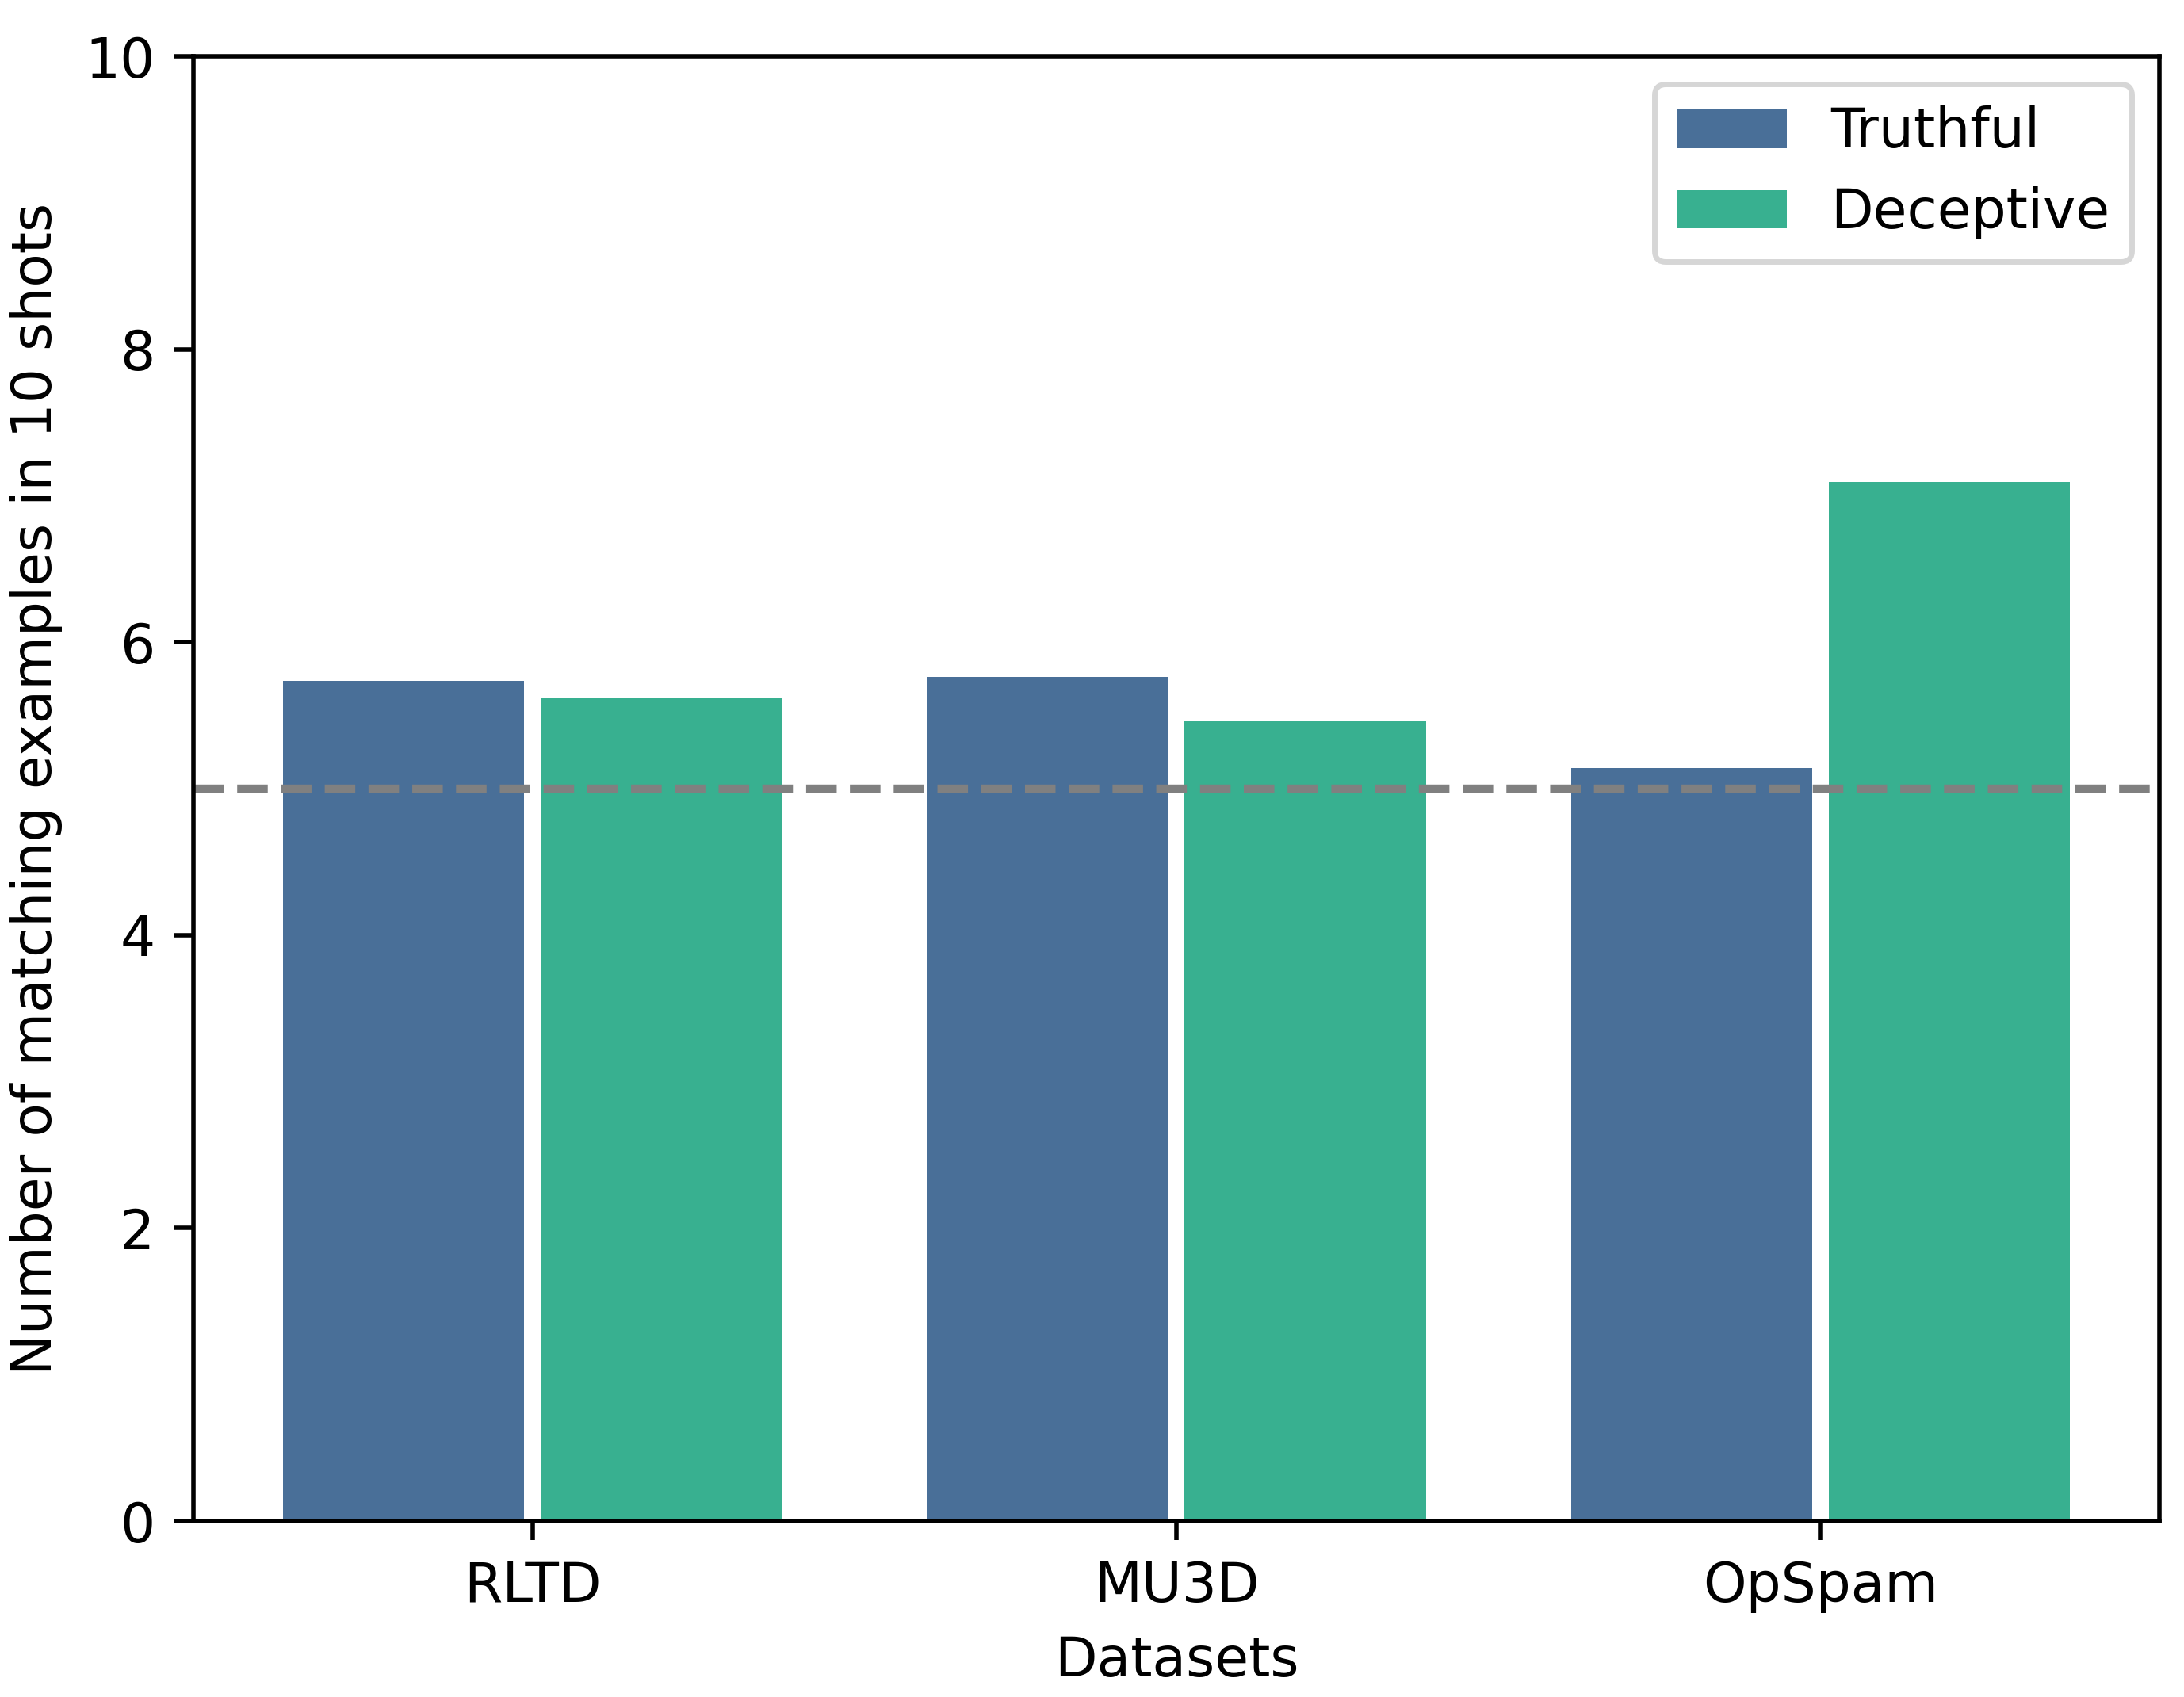
\includegraphics[width=0.45\textwidth]{images/dc_num_examples.png}
    % \captionsetup{font=scriptsize}
    \caption{Average number of matching examples in 10-shot for sim-top strategy.}
    \label{fig:num_example}
\end{figure}

Looking closely at RLTD, the sim-pair approach slightly outperforms sim-top. In contrast, on MU3D and OpSpam, sim-top provides superior results, particularly on OpSpam, where the average F1 score improvement, $\sim4\%$, is notably higher than that observed on MU3D $\sim2\%$. Figure~\ref{fig:num_example} further illuminates these findings by illustrating the average number of `matching' examples (i.e., truthful examples for a truthful query and deceptive examples for a deceptive query) retrieved in a 10-shot setup using sim-top. For RLTD and MU3D, this number hovers around five, effectively mirroring the label balance of sim-pair. However, in OpSpam, especially for the deceptive queries, the average number of retrieved deceptive examples rises to about 7.1, enabling a substantial boost in performance. Concretely, this increase in label-specific examples elevates the deceptive-class F1 score from approximately 67\% under sim-pair to 73\% under sim-top. This finding also suggests that deceptive reviews in the OpSpam dataset exhibit a higher degree of semantic similarity compared to the other datasets, hence easily identifiable by the retriever.

\subsection{Impacts of Auxiliary Features}

\begin{table}
\centering
\small
\begin{tabular}{l c c cc cc}
\toprule
\textbf{LLM} & \textbf{Feats} & \textbf{Config} 
  & \multicolumn{2}{c}{\textbf{RLTD}} 
  & \multicolumn{2}{c}{\textbf{MU3D}} \\
\cmidrule(lr){4-5}\cmidrule(lr){6-7}
 & & & \textbf{Acc} & \textbf{F1} & \textbf{Acc} & \textbf{F1} \\
\midrule

% -----------------------
% Llama-3.1-8B
% -----------------------
\multirow{6}{*}{LLaMA 3.1} 
 & \multirow{2}{*}{\textit{non-verbal}}
   & \textit{zero-shot}
     & 51.24 & 35.34 
     & - & -  \\
 & 
   & \textit{\textit{few-shot}}
     & 63.02 & 62.79
     & - & -  \\
\cmidrule(lr){2-7}
 & \multirow{2}{*}{\textit{video summaries}}
   & \textit{zero-shot}
     & 52.07 & 38.40
     & 50.63 & 49.67 \\
 &
   & \textit{\textit{few-shot}}
     & 62.60 & 61.72 
     & 51.88 & 49.44 \\
\cmidrule(lr){2-7}
 & \multirow{2}{*}{\textit{audio summaries}}
   & \textit{zero-shot}
     & 57.85 & 57.56
     & 49.06 & 49.00 \\
 &
   & \textit{\textit{few-shot}}
     & 64.74 & 63.12
     & 51.57 & 51.25 \\
\midrule

% -----------------------
% Gemma2-9B
% -----------------------
\multirow{6}{*}{Gemma 2} 
 & \multirow{2}{*}{\textit{non-verbal}}
   & \textit{zero-shot}
     & 52.07 & 38.40 
     & - & -  \\
 & 
   & \textit{\textit{few-shot}}
     & 66.67 & 64.85
     & - & -  \\
\cmidrule(lr){2-7}
 & \multirow{2}{*}{\textit{video summaries}}
   & \textit{zero-shot}
     & 52.07 & 38.40 
     & 51.25 & 44.16 \\
 &
   & \textit{\textit{few-shot}}
     & 66.94 & 66.92 
     & \textbf{53.44} & \textbf{51.56} \\
\cmidrule(lr){2-7}
 & \multirow{2}{*}{\textit{audio summaries}}
   & \textit{zero-shot}
     & 66.94 & 66.28
     & 49.38 & 45.82 \\
 &
   & \textit{\textit{few-shot}}
     & 68.60 & 68.59
     & 51.56 & 50.98 \\
\midrule

% -----------------------
% GPT-4o
% -----------------------
\multirow{6}{*}{GPT-4o} 
 & \multirow{2}{*}{\textit{non-verbal}}
   & \textit{zero-shot}
     & 65.29 & 61.71
     & - & -  \\
 & 
   & \textit{\textit{few-shot}}
     & \textbf{72.93} & \textbf{72.84} 
     & - & -  \\
\cmidrule(lr){2-7}
 & \multirow{2}{*}{\textit{video summaries}}
   & \textit{zero-shot}
     & 65.29 & 65.00
     & 52.19 & 47.98 \\
 &
   & \textit{\textit{few-shot}}
     & 69.42 & 69.00 
     & 54.69 & 52.48 \\
\cmidrule(lr){2-7}
 & \multirow{2}{*}{\textit{audio summaries}}
   & \textit{zero-shot}
     & 66.12 & 64.73
     & 49.38 & 42.31 \\
 &
   & \textit{\textit{few-shot}}
     & 67.69 & 66.85
     & 51.63 & 45.21 \\
\bottomrule
\end{tabular}

% \captionsetup{font=scriptsize}
\caption{Comparison of auxiliary features for the multimodal datasets.}
\label{tab:aux_features_multimodal}
\end{table}


In Table~\ref{tab:aux_features_multimodal}, we compare three types of auxiliary features: non-verbal gestures, LLM-generated audio and video summaries under both zero-shot and few-shot settings. Each model uses randomly selected in-context examples when operating in the few-shot configuration. From these results, we observe that including non-verbal gestures alongside the transcript yields a modest improvement for GPT-4o ($\sim1.4$ points in F1 score on the RLTD dataset). This gain is consistent with GPT-4o’s demonstrated strengths in in-context learning. In contrast, the inclusion of non-verbal features negatively impacts LLaMA 3.1 and Gemma 2: their tendency to overpredict the \texttt{Deceptive} label suggests that limited in-context examples are insufficient for these models to learn patterns of non-verbal gestures across truthful and deceptive scenarios. Turning to video summaries, GPT-4o again exhibits relative gains on MU3D, although the improvements for other models and datasets remain negligible or even degrade performance. A similar pattern holds for audio summaries: while certain configurations see a slight boost, many are on par with or slightly below the corresponding transcript-only results. 
Overall, additional features do not universally enhance predictive accuracy without fine-tuning.


\section{Summary}
Our comprehensive evaluation reveals that LLMs and LMMs exhibit promising capabilities for deception detection across diverse contexts. While fine-tuning significantly enhanced performance, improvements on multimodal datasets are still lagging, highlighting persistent challenges in capturing nuanced cross-modal deception cues in LMMs. Moreover, incorporating reasoning generation to explain predictions did not consistently improve overall accuracy over straightforward label prediction, emphasizing that the inherently ambiguous nature of deception cues makes it harder for the models to reason successfully. These findings underscore the importance of careful prompt design and in-context example selection while pointing to the need for further methodological refinements in practical deception detection applications.